\FloatBarrier
\section{UK vs.\ U.S.}\label{app:UKUS}\setcounter{equation}{0}
Sections \ref{sec:oecd} and \ref{sec:esc} impose France's income distribution, leisure preferences and voting patterns on the U.S.\ model. This appendix reports those counterfactuals in full and repeats them with the UK as the host economy, first with the pension design held at the host's value and then with the design chosen by the electorate.

\subsection{French characteristics given the pension design}\label{app:US:french}

Table \ref{table:US:otherShocks} reports the counterfactuals of section \ref{sec:oecd} that impose France's income distribution, leisure preferences and voting patterns on the U.S.\ model, one at a time and all at once, next to France's own calibrated path. Table \ref{table:US:CRRA:otherShocks} repeats them under general CRRA preferences.
Section \ref{sec:oecd} discusses the first. In the second, the effect of France's income distribution shrinks as the elasticity rises, from a fall in the tax rate of $1.6$ p.p.\ at $\rho = 0.5$ to $0.8$ p.p.\ at $\rho = 2$, while the effect of its voting profile grows, from a rise of $0.3$ p.p.\ to $1.7$ p.p.; section \ref{sec:oecd} gives the reason for the second.

%% GENERATED by python/paper/build.py from results/ -- do not edit by hand.
%% Rebuild:  .venv\Scripts\python.exe python\paper\build.py --only US_OtherShocks
%% Source:   results/shocks/US_shocksCommonX.csv
\begin{table}[!htb]
\centering
\begin{threeparttable}
\caption{French income distribution and voting patterns in US}
\label{table:US:otherShocks}
\renewcommand{\arraystretch}{1.25}
\begin{tabularx}{.9\textwidth}{lYYY}
\toprule
\textbf{Scenario} & \textbf{Tax rate} & \textbf{Savings rate} & \textbf{Avg. workweek} \\
\midrule 
Baseline & 14.43\% & 15.37\% & 39.39 \\
Income distribution & 13.21\% & $+0.44$ p.p. & 40.36 \\
Voting & 15.32\% & $-0.32$ p.p. & 39.19 \\
All French characteristics & 13.85\% & $+0.21$ p.p. & 35.29 \\[.5em]\hline\\[-.75em]
France (own calibration) & 21.29\% & $-1.94$ p.p. & 35.44 \\
\bottomrule
\end{tabularx}
\begin{tablenotes}[flushleft]
\footnotesize
\item[] \textit{Note:} $\rho = 1.0$, full effect. Each row is a separate equilibrium path: the borrowed characteristics hold throughout and the economy starts from its own steady state, so the row describes a country that has always had this mix rather than the US hit by a surprise in 2020. Income distribution replaces $\eta_i$ with France\textquotesingle s while holding $X_i$ \emph{and} holding $\theta$ at the US design, so it is a change in inequality alone; pension design is the separate counterfactual of Table~\ref{table:US:pensChars}. All French characteristics imposes France\textquotesingle s $\eta_i$, voting weights $\mu_i$ and level of $X_i$ at once; the last, a pure rescaling of the hours unit, moves hours and nothing else. The last row is France\textquotesingle s own calibrated path, its savings rate reported as the distance from the US baseline.
\end{tablenotes}
\end{threeparttable}
\end{table}


%% GENERATED by python/paper/build.py from results/ -- do not edit by hand.
%% Rebuild:  .venv\Scripts\python.exe python\paper\build.py --only US_CRRA_OtherShocks
%% Source:   results/shocks/US_shocksCommonX.csv
\begin{table}[!htb]
\centering
\begin{threeparttable}
\caption{Does CRRA matter for French characteristics imposed on the US -- 2020}
\label{table:US:CRRA:otherShocks}
\renewcommand{\arraystretch}{1.25}
\begin{tabularx}{.9\textwidth}{YYYYY}
\toprule
\textbf{Scenario} & \textbf{CRRA} ($\rho$) & \textbf{Tax rate} & \textbf{Savings rate} & \textbf{Avg. workweek} \\
\midrule 
 & 0.5 & 14.43\% & 15.91\% & 39.39 \\
Baseline & 1.0 & 14.43\% & 15.37\% & 39.39 \\
 & 2.0 & 14.43\% & 14.85\% & 39.39 \\[.5em]\hline\\[-.75em]
 & 0.5 & 12.88\% & $+0.83$ p.p. & 40.53 \\
Income distribution & 1.0 & 13.21\% & $+0.44$ p.p. & 40.36 \\
 & 2.0 & 13.65\% & $+0.16$ p.p. & 40.22 \\[.5em]\hline\\[-.75em]
 & 0.5 & 14.75\% & $-0.17$ p.p. & 39.30 \\
Voting & 1.0 & 15.32\% & $-0.32$ p.p. & 39.19 \\
 & 2.0 & 16.12\% & $-0.34$ p.p. & 39.11 \\[.5em]\hline\\[-.75em]
\bottomrule
\end{tabularx}
\begin{tablenotes}[flushleft]
\footnotesize
\item[] \textit{Note:} Every $\rho$ is separately calibrated. Every scenario row reports the change in the savings rate against the baseline at the same $\rho$, in percentage points.
\end{tablenotes}
\end{threeparttable}
\end{table}


The same characteristics can be imposed on the UK, with France's households regrouped at the UK's income cuts (appendix \ref{app:US:calibFRUK}). Tables \ref{table:UK:otherShocks} and \ref{table:UK:CRRA:otherShocks} report the counterfactuals on the UK's own calibration, with $\theta$ held at the UK's value in the income-distribution row as in the U.S.\ exercise. France's income distribution raises the UK's tax rate by 0.3 p.p., where it lowers the U.S.\ one by 1.2 p.p. The reason for this is that at the UK's cuts France is the more unequal of the two countries (table \ref{table:a_US:CalibFRUK}): borrowing France's distribution raises inequality in the UK, and equilibrium taxes increase with inequality (proposition \ref{prop:LOG:PEE}). France's voting patterns raise the tax by 0.3 p.p., as in the U.S., since France's voting profile is flatter than the UK's and the poor gain weight. Leisure preferences leave every rate unchanged and lengthen the workweek by 1.1 hours, France's average taste for leisure being below the UK's. All three at once raise the tax rate by 0.6 p.p.\ and take the workweek to 35.6 hours, against France's own 35.2; the remaining 8.8 p.p.\ between the UK's 12.5\% and France's 21.3\% is France's demography, its fully Bismarckian design and the political weight of its old, as in the U.S.\ exercise. Across $\rho$ the income-distribution and voting effects stay between 0.1 and 0.5 p.p., and the savings rate moves by less than 0.3 p.p.\ of GDP in every row. The income-distribution row is the one that depends on the calibration variant: under the vector-$X_i$ calibration (table \ref{table:UK:otherShocks_vectorX}) it lowers the UK's tax rate by 0.5 p.p.\ instead, because that variant reads part of the observed income dispersion off relative hours, which are much flatter in the UK than in France, and so attributes a different productivity distribution to each country.

%% GENERATED by python/paper/build.py from results/ -- do not edit by hand.
%% Rebuild:  .venv\Scripts\python.exe python\paper\build.py --only UK_OtherShocks
%% Source:   results/shocks/UK_shocksCommonX.csv
\begin{table}[!htb]
\centering
\begin{threeparttable}
\caption{French income distribution, leisure preferences and voting patterns in the UK}
\label{table:UK:otherShocks}
\renewcommand{\arraystretch}{1.25}
\begin{tabularx}{.9\textwidth}{lYYY}
\toprule
\textbf{Scenario} & \textbf{Tax rate} & \textbf{Savings rate} & \textbf{Avg. workweek (hours)} \\
\midrule 
Baseline & 11.86\% & 17.20\% & 34.73 \\ % row: baseline
Income distribution & 12.15\% & $-0.12$ p.p. & 34.55 \\ % row: income
Leisure preferences & 11.86\% & 0.00 p.p. & 35.85 \\ % row: leisure
Voting patterns & 12.19\% & $-0.13$ p.p. & 34.66 \\ % row: voting
All French characteristics & 12.46\% & $-0.24$ p.p. & 35.61 \\[.5em]\hline\\[-.75em] % row: frall
France (own calibration) & 21.29\% & $-3.76$ p.p. & 35.24 \\ % row: france
\bottomrule
\end{tabularx}
\begin{tablenotes}[flushleft]
\footnotesize
\item[] \textit{Note:} $\rho = 1.0$, full effect. Each row is a separate equilibrium path: the borrowed characteristics hold throughout and the economy starts from its own steady state, so the row describes a country that has always had this mix rather than the UK hit by a surprise in 2020. Income distribution replaces $\eta_i$ with France\textquotesingle s while holding $X_i$ and $\theta$ at their UK values, so it is a change in inequality alone. Leisure preferences keeps the UK $\eta_i$ and rescales every $X_i$ to France\textquotesingle s population-weighted mean $X$, scaled as France\textquotesingle s $\eta_i$ are in the income row; it is a pure rescaling of the hours unit and moves hours and nothing else. All French characteristics imposes France\textquotesingle s $\eta_i$, level of $X_i$ and voting weights $\mu_i$ at once. The last row is France\textquotesingle s own calibrated path, its savings rate reported as the distance from the UK baseline. France\textquotesingle s income groups are cut at the UK\textquotesingle s own income percentiles here (table \ref{table:a_US:CalibFRUK}).
\end{tablenotes}
\end{threeparttable}
\end{table}


%% GENERATED by python/paper/build.py from results/ -- do not edit by hand.
%% Rebuild:  .venv\Scripts\python.exe python\paper\build.py --only UK_CRRA_OtherShocks
%% Source:   results/shocks/UK_shocksCommonX.csv
\begin{table}[!htb]
\centering
\begin{threeparttable}
\caption{Does CRRA matter for French characteristics imposed on the UK -- 2020}
\label{table:UK:CRRA:otherShocks}
\renewcommand{\arraystretch}{1.25}
\begin{tabularx}{.9\textwidth}{YYYYY}
\toprule
\textbf{Scenario} & \textbf{CRRA} ($\rho$) & \textbf{Tax rate} & \textbf{Savings rate} & \textbf{Avg. workweek} \\
\midrule 
 & 0.5 & 11.86\% & 18.93\% & 34.73 \\ % row: baseline@0.5
Baseline & 1.0 & 11.86\% & 17.20\% & 34.73 \\ % row: baseline@1.0
 & 2.0 & 11.86\% & 15.80\% & 34.73 \\[.5em]\hline\\[-.75em] % row: baseline@2.0
 & 0.5 & 11.94\% & $-0.05$ p.p. & 34.59 \\ % row: income@0.5
Income distribution & 1.0 & 12.15\% & $-0.12$ p.p. & 34.55 \\ % row: income@1.0
 & 2.0 & 12.23\% & $-0.09$ p.p. & 34.55 \\[.5em]\hline\\[-.75em] % row: income@2.0
 & 0.5 & 12.08\% & $-0.14$ p.p. & 34.67 \\ % row: voting@0.5
Voting & 1.0 & 12.19\% & $-0.13$ p.p. & 34.66 \\ % row: voting@1.0
 & 2.0 & 12.39\% & $-0.12$ p.p. & 34.65 \\[.5em]\hline\\[-.75em] % row: voting@2.0
\bottomrule
\end{tabularx}
\begin{tablenotes}[flushleft]
\footnotesize
\item[] \textit{Note:} Every $\rho$ is separately calibrated. Every scenario row reports the change in the savings rate against the baseline at the same $\rho$, in percentage points.
\end{tablenotes}
\end{threeparttable}
\end{table}


Figure \ref{fig:UKUS:french} puts the two hosts side by side on common axes, at each $\rho$. Two differences stand out. France's income distribution moves the two tax rates in opposite directions at every elasticity, lowering the U.S.\ one and raising the UK's, for the reason given above. And France's taste for leisure shortens the U.S.\ workweek by about five hours but lengthens the UK's by about one, since France's average taste for leisure lies above the U.S.\ one and below the UK's. France's voting profile raises the tax rate on both hosts, by more at a higher elasticity, and on both the effects on the savings rate stay below $1$ p.p.\ of GDP.

\begin{figure}[!htb]
    \centering
    \caption{French characteristics in the U.S.\ and the UK}
    \label{fig:UKUS:french}
\begin{threeparttable}
    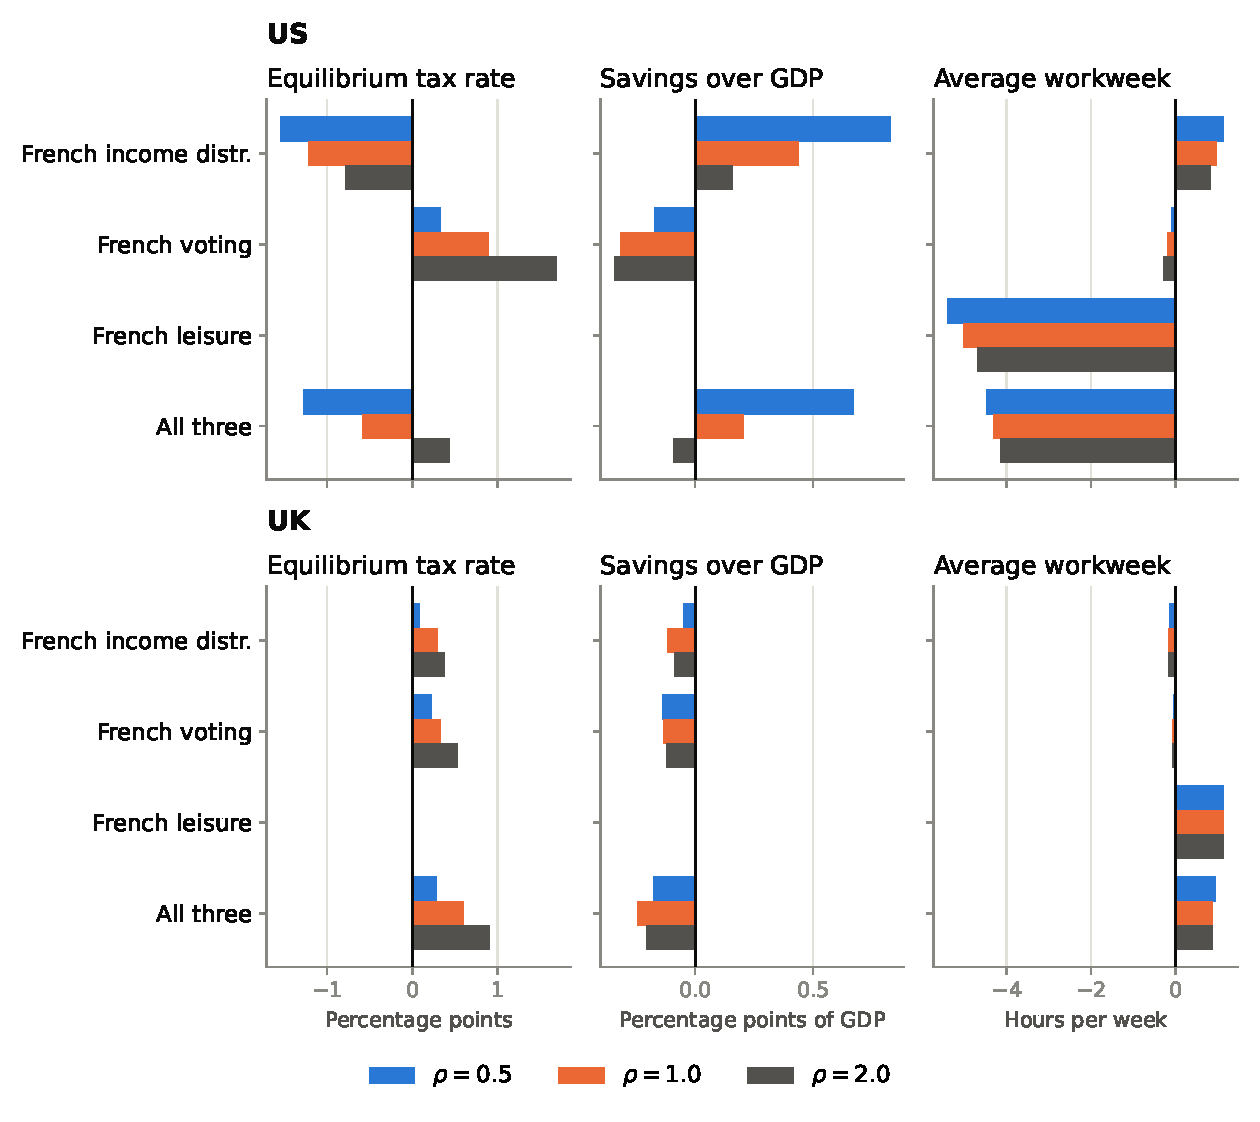
\includegraphics[width=\linewidth]{Figs/UKUS_French.pdf}
\begin{tablenotes}[flushleft]\footnotesize
    \item[] \textit{Note:} Every panel is the deviation from the host's own baseline at the same $\rho$, whose levels are the baseline rows of tables \ref{table:US:CRRA:otherShocks} and \ref{table:UK:CRRA:otherShocks}. France's income groups are cut at the host's income percentiles. The savings rate is savings relative to GDP.
\end{tablenotes}
\end{threeparttable}
\end{figure}

\FloatBarrier
\subsection{French characteristics with endogenous pension design}\label{app:US:ukESC}

Section \ref{sec:esc:calibration} calibrates the deadweight cost of redistribution on one datum, the U.S.\ design, and tests it on the UK and France (table \ref{table:US_ESC:country}). This appendix reports the counterfactuals of section \ref{sec:esc:results} with the design chosen, on the U.S.\ and then on the UK.

Tables \ref{table:US_ESC:incomeDistr} to \ref{table:US_ESC:frenchAll} report the counterfactuals of section \ref{sec:esc} that impose France's characteristics on the U.S., with the design pinned at the U.S.\ value and with the design chosen, at $\rho \in \{0.5, 1, 2\}$. France's income distribution moves the chosen design to $0.71$, $0.77$ and $0.92$ at $\rho = 0.5$, $1$ and $2$, its voting profile to $0.69$, $0.65$ and $0.33$, and all three characteristics together to $0.67$, $0.63$ and $0.26$; section \ref{sec:esc} discusses the mechanisms. At $\rho \leq 1$ the design response leaves the tax rate within $0.1$ p.p.\ of the pinned reading in all three tables. At $\rho = 2$, where the design moves furthest, the tax rate ends between $0.2$ and $0.6$ p.p.\ above it and the workweek up to half an hour below it.

%% GENERATED by python/paper/build.py from results/ -- do not edit by hand.
%% Rebuild:  .venv\Scripts\python.exe python\paper\build.py --only US_ESC_IncomeDistr
%% Source:   results/esc/escExperiments.csv
\begin{table}[!htb]
\centering
\begin{threeparttable}
\caption{Endogenous design and the French income distribution in US}
\label{table:US_ESC:incomeDistr}
\renewcommand{\arraystretch}{1.25}
\begin{tabularx}{\textwidth}{p{2.6cm}YYYYY}
\toprule
\textbf{Scenario} & \textbf{CRRA} ($\rho$) & $\bm{\theta}$ \textbf{(2020)} & \textbf{Tax rate} & \textbf{Savings rate} & \textbf{Avg. workweek} \\
\midrule 
 & 0.5 & 0.74 & 14.41\% & 16.10\% & 39.45 \\
Baseline & 1.0 & 0.74 & 14.43\% & 15.41\% & 39.47 \\
 & 2.0 & 0.74 & 14.44\% & 14.87\% & 39.42 \\[.5em]\hline\\[-.75em]
 & 0.5 & 0.74 & 13.71\% & $+0.27$ p.p. & 40.30 \\
Exogenous $\theta$ & 1.0 & 0.74 & 13.78\% & $+0.25$ p.p. & 40.24 \\
 & 2.0 & 0.74 & 13.85\% & $+0.12$ p.p. & 40.19 \\[.5em]\hline\\[-.75em]
 & 0.5 & 0.71 & 13.67\% & $+0.24$ p.p. & 40.35 \\
Endogenous $\theta$ & 1.0 & 0.77 & 13.80\% & $+0.16$ p.p. & 40.34 \\
 & 2.0 & 0.92 & 14.09\% & 0.00 p.p. & 40.36 \\[.5em]\hline\\[-.75em]
 & 0.5 & 1.00 & 21.29\% & $-1.44$ p.p. & 35.24 \\
France & 1.0 & 1.00 & 21.29\% & $-1.97$ p.p. & 35.24 \\
 & 2.0 & 1.00 & 21.29\% & $-2.39$ p.p. & 35.24 \\[.5em]\hline\\[-.75em]
\bottomrule
\end{tabularx}
\begin{tablenotes}[flushleft]
\footnotesize
\item[] \textit{Note:} The cost specification and the units are those of table \ref{table:US_ESC:ageing}. The France row is France's own calibrated path rather than a counterfactual on the US model: it carries France\textquotesingle s own $\omega$ as well as its characteristics, and its workweek is a calibration target rather than a prediction.
\end{tablenotes}
\end{threeparttable}
\end{table}


%% GENERATED by python/paper/build.py from results/ -- do not edit by hand.
%% Rebuild:  .venv\Scripts\python.exe python\paper\build.py --only US_ESC_Voting
%% Source:   results/esc/escExperiments.csv
\begin{table}[!htb]
\centering
\begin{threeparttable}
\caption{Endogenous design and French voting patterns in US}
\label{table:US_ESC:voting}
\renewcommand{\arraystretch}{1.25}
\begin{tabularx}{\textwidth}{p{2.6cm}YYYYY}
\toprule
\textbf{Scenario} & \textbf{CRRA} ($\rho$) & $\bm{\theta}$ \textbf{(2020)} & \textbf{Tax rate} & \textbf{Savings rate} & \textbf{Avg. workweek} \\
\midrule 
 & 0.5 & 0.74 & 14.42\% & 15.98\% & 39.40 \\
Baseline & 1.0 & 0.74 & 14.43\% & 15.38\% & 39.40 \\
 & 2.0 & 0.74 & 14.43\% & 14.85\% & 39.40 \\[.5em]\hline\\[-.75em]
 & 0.5 & 0.74 & 14.78\% & $-0.17$ p.p. & 39.29 \\
Exogenous $\theta$ & 1.0 & 0.74 & 15.35\% & $-0.31$ p.p. & 39.19 \\
 & 2.0 & 0.74 & 16.13\% & $-0.34$ p.p. & 39.10 \\[.5em]\hline\\[-.75em]
 & 0.5 & 0.65 & 15.07\% & $-0.05$ p.p. & 39.18 \\
Endogenous $\theta$ & 1.0 & 0.53 & 15.93\% & $-0.22$ p.p. & 38.88 \\
 & 2.0 & 0.26 & 17.53\% & $-0.38$ p.p. & 38.30 \\[.5em]\hline\\[-.75em]
 & 0.5 & 1.00 & 21.29\% & $-1.32$ p.p. & 35.24 \\
France & 1.0 & 1.00 & 21.29\% & $-1.95$ p.p. & 35.24 \\
 & 2.0 & 1.00 & 21.29\% & $-2.38$ p.p. & 35.24 \\[.5em]\hline\\[-.75em]
\bottomrule
\end{tabularx}
\begin{tablenotes}[flushleft]
\footnotesize
\item[] \textit{Note:} The cost specification and the units are those of table \ref{table:US_ESC:ageing}. The France row is France's own calibrated path rather than a counterfactual on the US model: it carries France\textquotesingle s own $\omega$ as well as its characteristics, and its workweek is a calibration target rather than a prediction.
\end{tablenotes}
\end{threeparttable}
\end{table}


%% GENERATED by python/paper/build.py from results/ -- do not edit by hand.
%% Rebuild:  .venv\Scripts\python.exe python\paper\build.py --only US_ESC_FrenchAll
%% Source:   results/esc/escExperiments.csv
\begin{table}[!htb]
\centering
\begin{threeparttable}
\caption{Endogenous design and all French characteristics in US}
\label{table:US_ESC:frenchAll}
\renewcommand{\arraystretch}{1.25}
\begin{tabularx}{\textwidth}{p{2.6cm}YYYYY}
\toprule
\textbf{Scenario} & \textbf{CRRA} ($\rho$) & $\bm{\theta}$ \textbf{(2020)} & \textbf{Tax rate} & \textbf{Savings rate} & \textbf{Avg. workweek} \\
\midrule 
 & 0.5 & 0.74 & 14.41\% & 16.10\% & 39.45 \\
Baseline & 1.0 & 0.74 & 14.43\% & 15.41\% & 39.47 \\
 & 2.0 & 0.74 & 14.44\% & 14.87\% & 39.42 \\[.5em]\hline\\[-.75em]
 & 0.5 & 0.74 & 13.97\% & $+0.13$ p.p. & 34.66 \\
Exogenous $\theta$ & 1.0 & 0.74 & 14.40\% & $+0.03$ p.p. & 34.96 \\
 & 2.0 & 0.74 & 15.05\% & $-0.13$ p.p. & 35.22 \\[.5em]\hline\\[-.75em]
 & 0.5 & 0.67 & 13.95\% & $+0.13$ p.p. & 34.69 \\
Endogenous $\theta$ & 1.0 & 0.63 & 14.44\% & $+0.05$ p.p. & 34.93 \\
 & 2.0 & 0.26 & 15.44\% & $-0.06$ p.p. & 34.83 \\[.5em]\hline\\[-.75em]
 & 0.5 & 1.00 & 21.29\% & $-1.44$ p.p. & 35.24 \\
France & 1.0 & 1.00 & 21.29\% & $-1.97$ p.p. & 35.24 \\
 & 2.0 & 1.00 & 21.29\% & $-2.39$ p.p. & 35.24 \\[.5em]\hline\\[-.75em]
\bottomrule
\end{tabularx}
\begin{tablenotes}[flushleft]
\footnotesize
\item[] \textit{Note:} The cost specification and the units are those of table \ref{table:US_ESC:ageing}. The scenario replaces the US $\eta_i$, the level of $X_i$ and the voting weights $\mu_i$ with France\textquotesingle s simultaneously. The France row is France's own calibrated path rather than a counterfactual on the US model: it carries France\textquotesingle s own $\omega$ as well as its characteristics, and its workweek is a calibration target rather than a prediction.
\end{tablenotes}
\end{threeparttable}
\end{table}


Tables \ref{table:UK_ESC:incomeDistr} to \ref{table:UK_ESC:frenchAll} repeat the exercise on the UK, with France's households cut at the UK's income groups and the cost parameter calibrated, as for the U.S., so that the UK electorate re-elects its own observed design, $0.560$. That parameter is $15.089$, $7.264$ and $2.786$ at $\rho = 0.5$, $1$ and $2$, against $18.242$, $8.643$ and $1.728$ for the U.S.\ (table \ref{table:US_ESC:calibration}): below the U.S.\ value at $\rho \leq 1$ and above it at $\rho = 2$. France's voting profile pushes the UK's design toward flat benefits at every elasticity, to $0.51$, $0.52$ and $0.43$, as it does the U.S.\ design, but by less: the fall is of the same size at $\rho = 0.5$, about half the U.S.\ one at $\rho = 1$ and a third at $\rho = 2$. The UK's own voting profile is already flatter than the U.S.\ one (appendix \ref{app:US}), so France's shifts less weight toward the poor. France's income distribution moves the two hosts' designs in opposite directions at every elasticity: the UK's to $0.57$, $0.55$ and $0.50$, the U.S.\ one to $0.71$, $0.77$ and $0.92$. The reason for this is the ranking of appendix \ref{app:US:calibFRUK}. On the U.S.\ France's distribution compresses relative incomes and on the UK it spreads them, so the small net effect of the redistributive stakes and the cost of carrying them, whose sign depends on the elasticity, reverses between the two hosts. Together with France's level of $X_i$, the two characteristics put the UK's design at $0.56$, $0.52$ and $0.41$, the voting profile prevailing at $\rho \geq 1$. The design response leaves the UK's tax rate within $0.05$ p.p.\ of the pinned reading in every row and at every elasticity, and its savings rate and workweek within $0.1$ of it, so on the UK the design response is confined to the design itself.

%% GENERATED by python/paper/build.py from results/ -- do not edit by hand.
%% Rebuild:  .venv\Scripts\python.exe python\paper\build.py --only UK_ESC_IncomeDistr
%% Source:   results/esc/escExperimentsUK.csv
\begin{table}[!htb]
\centering
\begin{threeparttable}
\caption{Endogenous design and the French income distribution in the UK}
\label{table:UK_ESC:incomeDistr}
\renewcommand{\arraystretch}{1.25}
\begin{tabularx}{\textwidth}{p{2.6cm}YYYYY}
\toprule
\textbf{Scenario} & \textbf{CRRA} ($\rho$) & $\bm{\theta}$ \textbf{(2020)} & \textbf{Tax rate} & \textbf{Savings rate} & \textbf{Avg. workweek} \\
\midrule 
 & 0.5 & 0.560 & 11.86\% & 19.11\% & 34.73 \\
Baseline & 1.0 & 0.560 & 11.86\% & 17.25\% & 34.75 \\
 & 2.0 & 0.560 & 11.86\% & 15.81\% & 34.74 \\[.5em]\hline\\[-.75em]
 & 0.5 & 0.560 & 11.79\% & $+0.11$ p.p. & 34.63 \\
Exogenous $\theta$ & 1.0 & 0.560 & 12.03\% & $-0.03$ p.p. & 34.58 \\
 & 2.0 & 0.560 & 12.14\% & $-0.06$ p.p. & 34.56 \\[.5em]\hline\\[-.75em]
 & 0.5 & 0.573 & 11.81\% & $+0.03$ p.p. & 34.63 \\
Endogenous $\theta$ & 1.0 & 0.551 & 12.02\% & $-0.04$ p.p. & 34.59 \\
 & 2.0 & 0.500 & 12.12\% & $-0.03$ p.p. & 34.53 \\[.5em]\hline\\[-.75em]
 & 0.5 & 1.000 & 21.29\% & $-4.45$ p.p. & 35.24 \\
France & 1.0 & 1.000 & 21.29\% & $-3.81$ p.p. & 35.24 \\
 & 2.0 & 1.000 & 21.29\% & $-3.34$ p.p. & 35.24 \\[.5em]\hline\\[-.75em]
\bottomrule
\end{tabularx}
\begin{tablenotes}[flushleft]
\footnotesize
\item[] \textit{Note:} The cost specification and the units are those of table \ref{table:US_ESC:ageing}, at the UK\textquotesingle s own cost parameter, calibrated per $\rho$ so that the UK electorate re-elects its observed design $\theta^{\ast} = 0.560$: $\lambda = 15.089, 7.264, 2.786$ at $\rho = 0.5, 1.0, 2.0$, with $\beta$ imposed from the US and $\omega$ recalibrated at each trial value. France\textquotesingle s income groups are cut at the UK\textquotesingle s own income percentiles (table \ref{table:a_US:CalibFRUK}). The France row is France's own calibrated path rather than a counterfactual on the UK model: it carries France\textquotesingle s own $\omega$ as well as its characteristics, and its workweek is a calibration target rather than a prediction.
\end{tablenotes}
\end{threeparttable}
\end{table}


%% GENERATED by python/paper/build.py from results/ -- do not edit by hand.
%% Rebuild:  .venv\Scripts\python.exe python\paper\build.py --only UK_ESC_Voting
%% Source:   results/esc/escExperimentsUK.csv
\begin{table}[!htb]
\centering
\begin{threeparttable}
\caption{Endogenous design and French voting patterns in the UK}
\label{table:UK_ESC:voting}
\renewcommand{\arraystretch}{1.25}
\begin{tabularx}{\textwidth}{p{2.6cm}YYYYY}
\toprule
\textbf{Scenario} & \textbf{CRRA} ($\rho$) & $\bm{\theta}$ \textbf{(2020)} & \textbf{Tax rate} & \textbf{Savings rate} & \textbf{Avg. workweek} \\
\midrule 
 & 0.5 & 0.560 & 11.86\% & 19.11\% & 34.73 \\ % row: baseline@0.5
Baseline & 1.0 & 0.560 & 11.86\% & 17.25\% & 34.75 \\ % row: baseline@1.0
 & 2.0 & 0.560 & 11.86\% & 15.81\% & 34.74 \\[.5em]\hline\\[-.75em] % row: baseline@2.0
 & 0.5 & 0.560 & 12.06\% & $-0.08$ p.p. & 34.68 \\ % row: pinned@0.5
Exogenous $\theta$ & 1.0 & 0.560 & 12.16\% & $-0.09$ p.p. & 34.67 \\ % row: pinned@1.0
 & 2.0 & 0.560 & 12.36\% & $-0.11$ p.p. & 34.65 \\[.5em]\hline\\[-.75em] % row: pinned@2.0
 & 0.5 & 0.511 & 12.02\% & $-0.08$ p.p. & 34.69 \\ % row: chosen@0.5
Endogenous $\theta$ & 1.0 & 0.521 & 12.15\% & $-0.08$ p.p. & 34.66 \\ % row: chosen@1.0
 & 2.0 & 0.426 & 12.37\% & $-0.09$ p.p. & 34.60 \\[.5em]\hline\\[-.75em] % row: chosen@2.0
 & 0.5 & 1.000 & 21.29\% & $-4.45$ p.p. & 35.24 \\ % row: france@0.5
France & 1.0 & 1.000 & 21.29\% & $-3.81$ p.p. & 35.24 \\ % row: france@1.0
 & 2.0 & 1.000 & 21.29\% & $-3.34$ p.p. & 35.24 \\[.5em]\hline\\[-.75em] % row: france@2.0
\bottomrule
\end{tabularx}
\begin{tablenotes}[flushleft]
\footnotesize
\item[] \textit{Note:} The cost specification, the cost parameter and the units are those of table \ref{table:UK_ESC:incomeDistr}. The France row is France's own calibrated path rather than a counterfactual on the UK model: it carries France\textquotesingle s own $\omega$ as well as its characteristics, and its workweek is a calibration target rather than a prediction.
\end{tablenotes}
\end{threeparttable}
\end{table}


%% GENERATED by python/paper/build.py from results/ -- do not edit by hand.
%% Rebuild:  .venv\Scripts\python.exe python\paper\build.py --only UK_ESC_FrenchAll
%% Source:   results/esc/escExperimentsUK.csv
\begin{table}[!htb]
\centering
\begin{threeparttable}
\caption{Endogenous design and all French characteristics in the UK}
\label{table:UK_ESC:frenchAll}
\renewcommand{\arraystretch}{1.25}
\begin{tabularx}{\textwidth}{p{2.6cm}YYYYY}
\toprule
\textbf{Scenario} & \textbf{CRRA} ($\rho$) & $\bm{\theta}$ \textbf{(2020)} & \textbf{Tax rate} & \textbf{Savings rate} & \textbf{Avg. workweek} \\
\midrule 
 & 0.5 & 0.56 & 11.86\% & 19.11\% & 34.73 \\
Baseline & 1.0 & 0.56 & 11.86\% & 17.25\% & 34.75 \\
 & 2.0 & 0.56 & 11.86\% & 15.81\% & 34.74 \\[.5em]\hline\\[-.75em]
 & 0.5 & 0.56 & 11.97\% & 0.00 p.p. & 35.75 \\
Exogenous $\theta$ & 1.0 & 0.56 & 12.31\% & $-0.14$ p.p. & 35.66 \\
 & 2.0 & 0.56 & 12.63\% & $-0.17$ p.p. & 35.63 \\[.5em]\hline\\[-.75em]
 & 0.5 & 0.56 & 11.98\% & $-0.05$ p.p. & 35.76 \\
Endogenous $\theta$ & 1.0 & 0.52 & 12.30\% & $-0.13$ p.p. & 35.65 \\
 & 2.0 & 0.41 & 12.64\% & $-0.12$ p.p. & 35.53 \\[.5em]\hline\\[-.75em]
 & 0.5 & 1.00 & 21.29\% & $-4.45$ p.p. & 35.24 \\
France & 1.0 & 1.00 & 21.29\% & $-3.81$ p.p. & 35.24 \\
 & 2.0 & 1.00 & 21.29\% & $-3.34$ p.p. & 35.24 \\[.5em]\hline\\[-.75em]
\bottomrule
\end{tabularx}
\begin{tablenotes}[flushleft]
\footnotesize
\item[] \textit{Note:} The cost specification, the cost parameter and the units are those of table \ref{table:UK_ESC:incomeDistr}. The scenario replaces the UK $\eta_i$, the level of $X_i$ and the voting weights $\mu_i$ with France\textquotesingle s simultaneously. The France row is France's own calibrated path rather than a counterfactual on the UK model: it carries France\textquotesingle s own $\omega$ as well as its characteristics, and its workweek is a calibration target rather than a prediction.
\end{tablenotes}
\end{threeparttable}
\end{table}


Figure \ref{fig:UKUS:escFrench} puts the two hosts side by side. On both, France's voting profile is the characteristic that moves the design most, and it moves it furthest at $\rho = 2$; there the move is three times larger on the U.S., whose calibrated cost at $\rho = 2$ is the lower of the two and whose voting profile is the steeper. On neither host does endogenizing the design move the tax rate by more than $0.1$ p.p.\ at $\rho \leq 1$.

\begin{figure}[!htb]
    \centering
    \caption{Endogenous pension design under French characteristics in the U.S.\ and the UK}
    \label{fig:UKUS:escFrench}
\begin{threeparttable}
    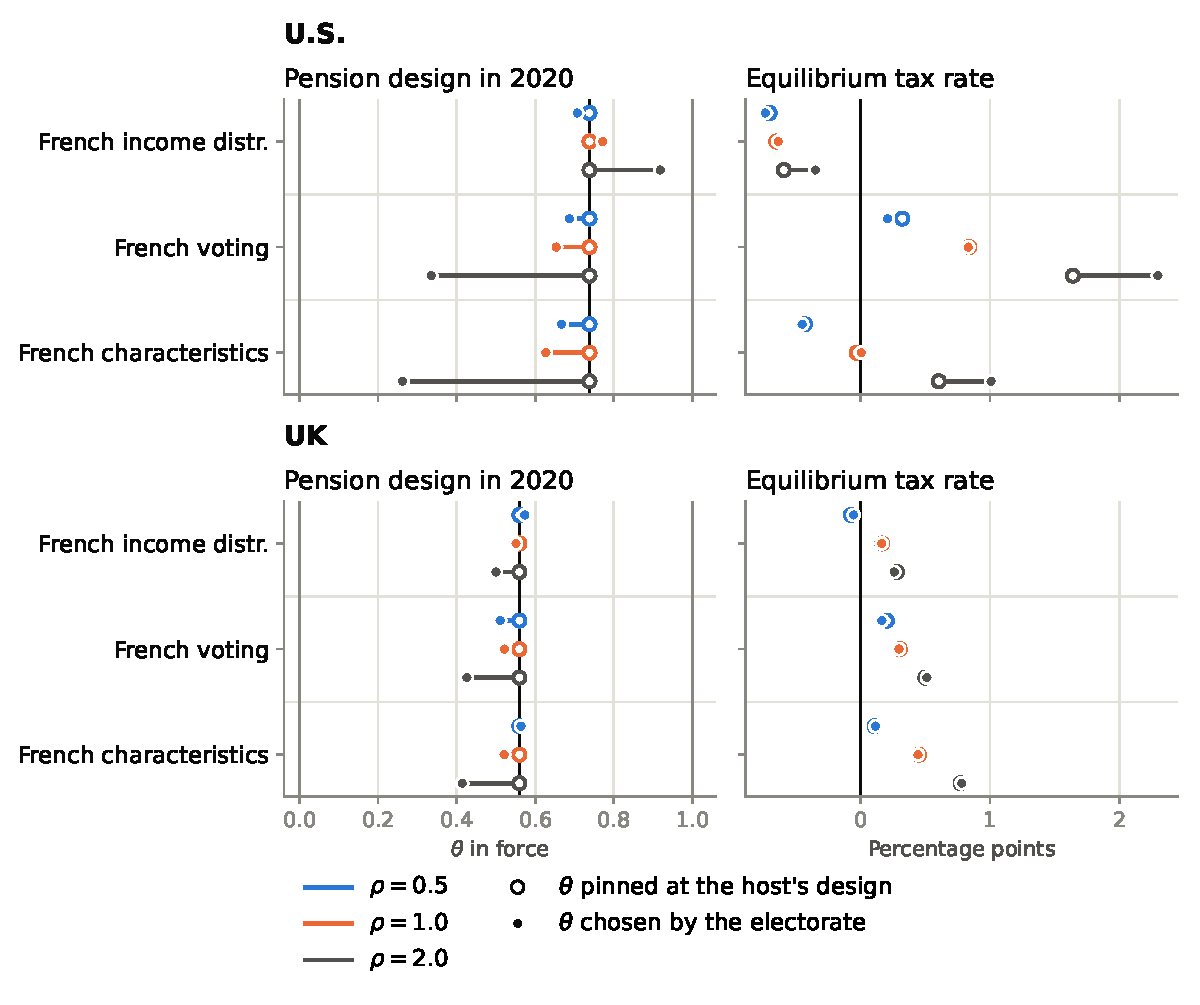
\includegraphics[width=\linewidth]{Figs/UKUS_ESC_French.pdf}
\begin{tablenotes}[flushleft]\footnotesize
    \item[] \textit{Note:} Each host at its own cost parameter (tables \ref{table:US_ESC:calibration} and \ref{table:UK_ESC:incomeDistr}). The first column is the design in force in 2020 as a level, the reference line at the host's observed design and the muted lines at the corners; the second is the tax rate as a deviation from the host's endogenous-$\theta$ baseline, whose levels are the baseline rows of tables \ref{table:US_ESC:incomeDistr} and \ref{table:UK_ESC:incomeDistr}. An open marker is the reading with the design pinned at the host's value, a filled one the reading with the design chosen.
\end{tablenotes}
\end{threeparttable}
\end{figure}
